\documentclass[xcolor=svgnames,english,presentation]{beamer}
%\documentclass[xcolor=svgnames,english,handout]{beamer}

%\usepackage{againframetitle}
%\aftOptions{style=NumberedLast}

\usepackage{graphics}
\usepackage{graphicx}
\usepackage{tabularx}

\usepackage{tikz}
\usepackage{pgfplots}

\graphicspath{{.}{pics/}}

% AALTO COLORS
\definecolor{aaltoyellow}{RGB}{254,203,00}  % FECB00
\definecolor{aaltored}{RGB}{237,41,57}      % ED2939
\definecolor{aaltoblue}{RGB}{00,101,189}    % 0065BD
\definecolor{aaltogray}{RGB}{146,139,129}   % 928B81
\definecolor{aaltolgreen}{RGB}{105,190,40}  % 69BE28
\definecolor{aaltodgreen}{RGB}{00,155,58}   % 009B3A
\definecolor{aaltocyan}{RGB}{00,168,180}    % 00A8B4
\definecolor{aaltopurple}{RGB}{102,57,183}  % 6639B7
\definecolor{aaltomagenta}{RGB}{177,05,157} % B1059D
\definecolor{aaltoorange}{RGB}{255,121,00}  % FF7900
\definecolor{aaltogreen}{RGB}{00,155,58}   % 009B3A

\useoutertheme{infolines} 
\setbeamertemplate{navigation symbols}{} 
%\usetheme{Marburg}
%\usetheme{Copenhagen}
%\usetheme{Frankfurt}
%\usetheme{Warsaw}
%\usetheme{Dresden}
\usetheme{Madrid}
%\setbeamercolor{structure}{fg=CadetBlue!90!black} 
\setbeamercolor{structure}{fg=aaltogreen!100!black} 
%\usecolortheme[overlystylish]{albatross}

\mode<presentation>
{
  \setbeamercovered{transparent}
}

\mode<handout>
{
  \beamertemplatesolidbackgroundcolor{black!5}
}

\usepackage[english]{babel}
%\usepackage[finnish]{babel}
% or whatever

\usepackage[latin1]{inputenc}
% or whatever

% \usepackage{times}
% \usepackage[T1]{fontenc}
% Or whatever. Note that the encoding and the font should match. If T1
% does not look nice, try deleting the line with the fontenc.

%\usepackage{amsmath,amsfonts}
%\usepackage[subscriptcorrection]{mtpro2}

\usepackage{upgreek}
\usepackage{amsmath,amsfonts,amssymb,amsthm}
% \usepackage{amsmath,amsfonts,amssymb,amsthm,mathrsfs}
% \usepackage{mathptmx}

\newcommand{\balert}[1]{\textcolor{blue}{#1}}


\title{Indoor positioning using smartphones}


%\subtitle
%{Presentation Subtitle} % (optional)

\author[Simo S\"arkk\"a]{Assoc.~Prof.~{\bf Simo S\"arkk\"a}}
% - Use the \inst{?} command only if the authors have different
%   affiliation.

\institute[EEA Department]{\balert{EEA Department / ELEC@Aalto, Finland}} % (optional, but mostly needed)

% - Use the \inst command only if there are several affiliations.
% - Keep it simple, no one is interested in your street address.

%\date[March 2, 2016]{\alert{Research Winter Day, March 2, 2016}}
\date{March 24, 2016}

%\subject{Talks}
% This is only inserted into the PDF information catalog. Can be left
% out. 

%%%%%%%%%%%%%%%%%%%%%%%%%%%%%%%%%%%%%%%%%
%
% macros begin
%
%%%%%%%%%%%%%%%%%%%%%%%%%%%%%%%%%%%%%%%%%

%\newtheorem{theorem}{Theorem}[section]
%\newtheorem{lemma}{Lemma}[section]
%\newtheorem{algorithm}{Algorithm}[section]
%\newtheorem{definition}{Definition}[section]
%\newtheorem{proposition}{Proposition}[section]
%\newtheorem{remark}{Remark}[section]
%\newtheorem{corollary}{Corollary}[section]
%\newtheorem{example}{Example}[section]

\newcommand{\T}[0]{\mathsf{T}}

\newcommand*{\diff}{\mathop{}\!\mathrm{d}}
\newcommand{\Dt}[0]{\delta t}
\newcommand{\Dx}[0]{\delta \vec{x}}
\newcommand{\Eg}[0]{\EuScript{E}}


\DeclareMathOperator{\tr}{tr}
\DeclareMathOperator{\diag}{diag}
\DeclareMathOperator{\chol}{chol}
\DeclareMathOperator{\dchol}{dchol}
\DeclareMathOperator{\Cov}{Cov}
\DeclareMathOperator{\Var}{Var}
\DeclareMathOperator{\E}{E}
\DeclareMathOperator{\N}{N}
\DeclareMathOperator{\gammad}{Gamma}
\DeclareMathOperator{\expd}{Exp}
\DeclareMathOperator{\sech}{sech}
\DeclareMathOperator{\KL}{KL}
\DeclareMathOperator{\U}{U}

\newcommand{\valpha}[0]{\boldsymbol{\alpha}}
\newcommand{\vbeta}[0]{\boldsymbol{\beta}}
\newcommand{\vchi}[0]{\boldsymbol{\chi}}
\newcommand{\vepsilon}[0]{\boldsymbol{\varepsilon}}
\newcommand{\veta}[0]{\boldsymbol{\eta}}
\newcommand{\vmu}[0]{\boldsymbol{\mu}}
\newcommand{\vphi}[0]{\boldsymbol{\phi}}
\newcommand{\vxi}[0]{\boldsymbol{\xi}}
\newcommand{\vtheta}[0]{\boldsymbol{\theta}}
\newcommand{\vTheta}[0]{\boldsymbol{\Theta}}
\newcommand{\vzeta}[0]{\boldsymbol{\zeta}}
\newcommand{\MPsi}[0]{\boldsymbol{\Psi}}
\newcommand{\MPhi}[0]{\boldsymbol{\Phi}}
\newcommand{\MSigma}[0]{\boldsymbol{\Sigma}}

\newcommand{\va}{\mathbf{a}}
\newcommand{\vb}{\mathbf{b}}
\newcommand{\vc}{\mathbf{c}}
\newcommand{\vd}{\mathbf{d}}
\newcommand{\ve}{\mathbf{e}}
\newcommand{\vf}{\mathbf{f}}
\newcommand{\vg}{\mathbf{g}}
\newcommand{\vh}{\mathbf{h}}
\newcommand{\vi}{\mathbf{i}}
\newcommand{\vj}{\mathbf{j}}
\newcommand{\vk}{\mathbf{k}}
\newcommand{\vl}{\mathbf{l}}
\newcommand{\vm}{\mathbf{m}}
\newcommand{\vn}{\mathbf{n}}
\newcommand{\vo}{\mathbf{o}}
\newcommand{\vp}{\mathbf{p}}
\newcommand{\vq}{\mathbf{q}}
\newcommand{\vr}{\mathbf{r}}
\newcommand{\vs}{\mathbf{s}}
\newcommand{\vu}{\mathbf{u}}
\newcommand{\vv}{\mathbf{v}}
\newcommand{\vw}{\mathbf{w}}
\newcommand{\vx}{\mathbf{x}}
\newcommand{\vy}{\mathbf{y}}
\newcommand{\vz}{\mathbf{z}}
\newcommand{\MA}{\mathbf{A}}
\newcommand{\MB}{\mathbf{B}}
\newcommand{\MC}{\mathbf{C}}
\newcommand{\MD}{\mathbf{D}}
\newcommand{\MF}{\mathbf{F}}
\newcommand{\MG}{\mathbf{G}}
\newcommand{\MH}{\mathbf{H}}
\newcommand{\MI}{\mathbf{I}}
\newcommand{\MJ}{\mathbf{J}}
\newcommand{\MK}{\mathbf{K}}
\newcommand{\ML}{\mathbf{L}}
\newcommand{\MM}{\mathbf{M}}
\newcommand{\MP}{\mathbf{P}}
\newcommand{\MQ}{\mathbf{Q}}
\newcommand{\MR}{\mathbf{R}}
\newcommand{\MS}{\mathbf{S}}
\newcommand{\MT}{\mathbf{T}}
\newcommand{\MV}{\mathbf{V}}
\newcommand{\MX}{\mathbf{X}}
\newcommand{\MY}{\mathbf{Y}}

\newcommand{\OL}{\mathscr{L}}


%%%%%%%%%%%%%%%%%%%%%%%%%%%%%%%%%%%%%%%%%
%
% macros end
%
%%%%%%%%%%%%%%%%%%%%%%%%%%%%%%%%%%%%%%%%%

% If you have a file called "university-logo-filename.xxx", where xxx
% is a graphic format that can be processed by latex or pdflatex,
% resp., then you can add a logo as follows:

%\pgfdeclareimage[height=0.5cm]{university-logo-small}{aalto_logo}
%\pgfdeclareimage[height=2cm]{university-logo-big}{aalto_logo}

% Delete this, if you do not want the table of contents to pop up at
% the beginning of each subsection:
\AtBeginSection[]
{
  \begin{frame}<beamer>
    \frametitle{Contents}
    \tableofcontents[currentsection]
  \end{frame}
}


% If you wish to uncover everything in a step-wise fashion, uncomment
% the following command: 

%\beamerdefaultoverlayspecification{<+->}

\begin{document}

%\logo{\pgfuseimage{university-logo-big}}

\begin{frame}
  \titlepage
\end{frame}

%\logo{\pgfuseimage{university-logo-small}}

\begin{frame}
  \frametitle{Contents}
  \tableofcontents[pausesections]
  % You might wish to add the option [pausesections]
\end{frame}

\section{Motivation}

\begin{frame}
  \frametitle{Why indoor positioning is important}

  % guidance
  % IoT
  % fire brigade
  % medical personnell

  \begin{columns}
  \begin{column}{0.7\textwidth}
  \begin{itemize}[<+->]

%  \item Indoor positioning has \alert{applications} in various areas.

  \item {\em Shopping mall applications:}
    \begin{itemize}[<+->]  
  	\item \alert{Wayfinding} in \balert{shopping malls}.
	\item Wayfinding and navigation in \alert{garages}.
  	\item Targeted \alert{advertisement} and \balert{analytics}.
    \end{itemize}
  \item {\em Hospitals}:
    \begin{itemize}[<+->]  
      \item Tracking of \alert{patients}.
      \item Alerting of \alert{medical personnel}. 
      \item Positioning of \alert{wireless medical equipment}. 
    \end{itemize}
  \item {\em Internet-of-things (IoT):}
    \begin{itemize}[<+->]    
      \item Positioning of \alert{IoT devices}.
      \item \alert{Ad-doc network} formation.
    \end{itemize}
  \item {\em Safety and security:}
    \begin{itemize}[<+->]    
      \item Navigation in \alert{burning buildings}.
      \item \alert{Security personnel} tracking.
    \end{itemize}
  \end{itemize}
  \end{column}
  \begin{column}{0.3\textwidth}
  \includegraphics[width=0.8\columnwidth]{nurse_nav} \\
  \includegraphics[width=0.8\columnwidth]{IoT} \\
  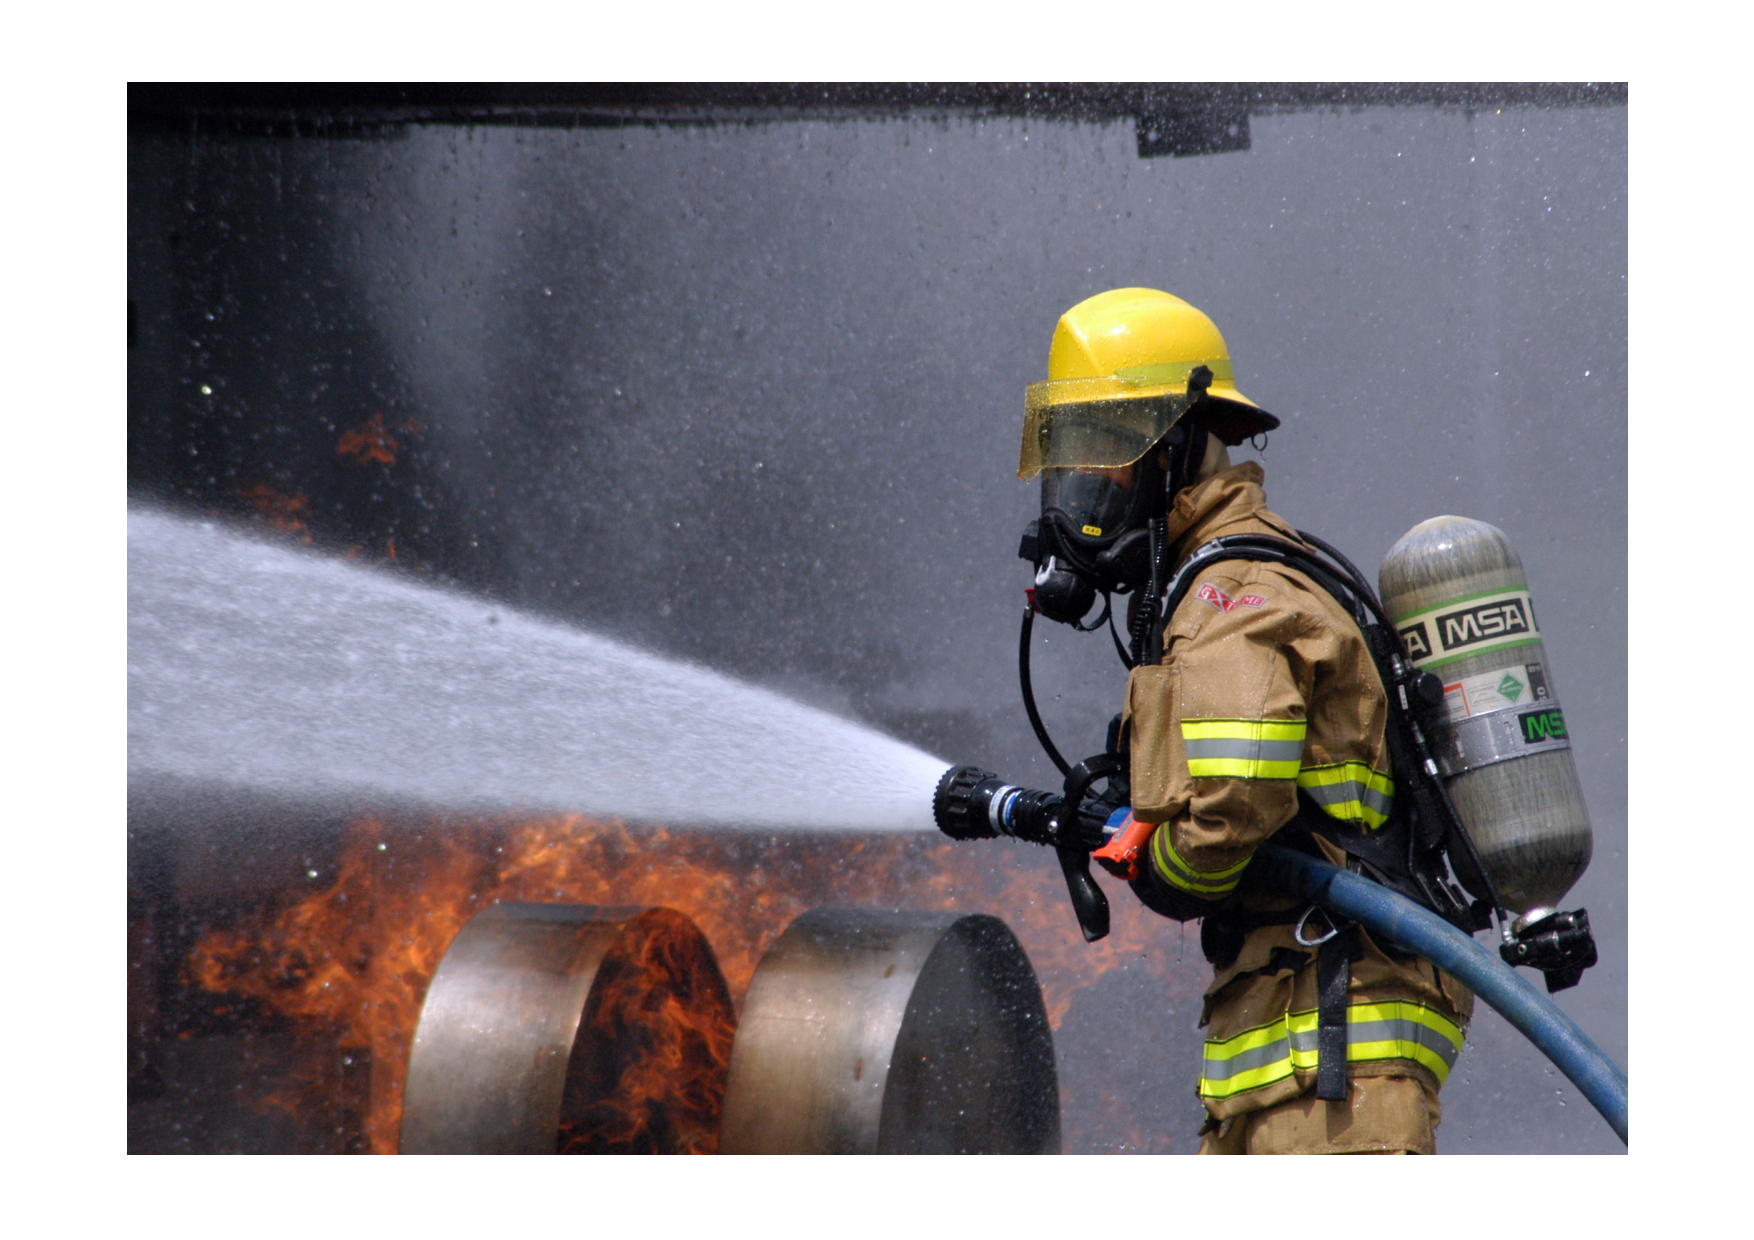
\includegraphics[width=0.8\columnwidth]{fire}
  \end{column}
  \end{columns}
\end{frame}

\begin{frame}
  \frametitle{Why indoor positioning is hard}

  % - 1m accuracy requirement
  % - GPS does not work indoors
  % - Different floors are significant
  \begin{columns}
  \begin{column}{0.7\textwidth}
  \begin{itemize}[<+->]       
  \item \alert{GPS does not work indoors} -- nor any other satellite navigation system.
  \item The \alert{accuracy requirement} is often \alert{1 meter}.
  \item \alert{Mobile phone network} positioning is not accurate enough.
  \item Accurate \alert{height} information is important (which floor).
  \item \alert{Indoor maps} can be challenging to obtain.
  \end{itemize}
  \end{column}
  \begin{column}{0.3\textwidth}
  \includegraphics[width=\columnwidth]{nogps} \\
  \includegraphics[width=\columnwidth]{accuracy} \\
  \includegraphics[width=\columnwidth]{floor}
  \end{column}
  \end{columns}
\end{frame}

\begin{frame}
  \frametitle{Sensors in modern smartphones}

  \begin{columns}
  \begin{column}{0.6\textwidth}
  \begin{itemize}[<+->]       
  \item \alert{GPS/GNSS receiver} for (outdoors) satellite positioning.
  \item \alert{Accelerometer and gyroscope} measure the local moment and rotation.
  \item \alert{WiFi, Bluetooth, and 3G/4G/5G} devices measure radio signals.
  \item \alert{Magnetometer} (compass) measures the local magnetic field direction.
  \item \alert{Barometer} measures the local pressure (gives information on height).
  \item \alert{Camera} measures the optical properties of the environment (i.e. takes pictures).
  \end{itemize}
  \end{column}
  \begin{column}{0.4\textwidth}
  \includegraphics[width=\columnwidth]{smartphone}
  \end{column}
  \end{columns}
\end{frame}

\section{Indoor positioning methods}

\begin{frame}
  \frametitle{WiFi and beacon-based positioning}

  \begin{columns}
  \begin{column}{0.6\textwidth}
  \begin{itemize}[<+->]       
  \item \alert{WiFi and (Bluetooth) beacons} are often used for indoor positioning.
  \item Based on measuring strengths of \alert{radio transmitters in known locations}.
  \item Requires building a \alert{map of the radio environment}.
  \item \alert{Accuracy} is limited by \alert{local attenuation and device differences}.
  \item \alert{Radio maps} need to be \alert{updated} continuously -- can be labour-intensive.
  \end{itemize}
  \end{column}
  \begin{column}{0.4\textwidth}
  \includegraphics[width=\columnwidth]{floorplan} \\
  \vspace{2em}
  \includegraphics[width=\columnwidth]{wifimap}
  \end{column}
  \end{columns}
\end{frame}

\begin{frame}
  \frametitle{Magnetic positioning}

  \begin{columns}
  \begin{column}{0.6\textwidth}
  \begin{itemize}[<+->]       
  \item \alert{Magnetic positioning} utilizes \alert{local magnetic field variations} in buildings.
  \item Requires creating a \alert{map of the magnetic field variations}.
  \item Due to field ambiguity, needs to be combined with \alert{inertial navigation} and \alert{orientation tracking}.
  \item \alert{Locally accurate}, benefits from \alert{combining with WiFi/Beacon positioning}.
  \end{itemize}
  \end{column}
  \begin{column}{0.4\textwidth}
  \includegraphics[width=\columnwidth]{terrain-matching} \\
  \vspace{2em}
  \includegraphics[width=\columnwidth]{magnetic}
  \end{column}
  \end{columns}
\end{frame}

\section{Sensor fusion and SLAM}

\begin{frame}
  \frametitle{Inertial navigation, PDRs, and orientation tracking}

  \begin{columns}
  \begin{column}{0.6\textwidth}
  \begin{itemize}[<+->]       
  \item \alert{Acceleration and angular velocity} can be \alert{integrated} to give position and orientation.
  \item Unknown \alert{initial conditions and sensors drifts} cause problems.
  \item The \alert{known gravitation direction} helps in \alert{orientation tracking}.
  \item Accelerometer can also be used to \alert{detect steps} -- gives a measurement of \alert{speed/distance}.
  \item \alert{Barometer} can be used to for \alert{local height tracking}. 
  \item Best when \alert{combined} with \alert{radio and magnetic} positioning methods.
  \end{itemize}
  \end{column}
  \begin{column}{0.4\textwidth}
  \includegraphics[width=\columnwidth]{mobile2} \\
  \includegraphics[width=\columnwidth]{grav}
  \end{column}
  \end{columns}
\end{frame}

\begin{frame}
  \frametitle{Simultaneous localization and mapping (SLAM)}

  \begin{columns}
  \begin{column}{0.5\textwidth}
  \begin{itemize}[<+->]       
  \item In \alert{simultaneous localization and mapping (SLAM)} the radio/ magnetic
  map is created while positioning.
  \item Considerably \alert{harder} than \alert{separate mapping and positioning}.
  \item Typically based on detecting a \alert{return to known location}:
  \begin{itemize}[<+->]       
  \item We can do a \alert{loop closure} to confirm the traveled path.
  \item \alert{Inertial navigation} can be used to map a small unknown area at a time.
  \item Known wall locations provide \alert{constraints}.
  \end{itemize}
  \end{itemize}
  \end{column}
  \begin{column}{0.5\textwidth}
  \includegraphics[width=\columnwidth]{slam} \\
  \end{column}
  \end{columns}
\end{frame}



\begin{frame}
  \frametitle{Gaussian processes, Kalman and particle filtering}

  \begin{columns}
  \begin{column}{0.65\textwidth}
  \begin{itemize}[<+->]       
  \item \alert{WiFi, beacon, and magnetic maps} typically estimated using \alert{Gaussian processes} (GPs).
  \item GPs are \alert{machine learning tools} for \alert{learning} the field from noisy observations.
  \item \alert{Inertial sensor fusion} is often done using \alert{(extended) Kalman filters}.
  \item \alert{Sensor fusion} with \alert{radio and magnetic} often done with \alert{particle filters}.
  \item When combined, can be used for \alert{simultaneous localization and mapping (SLAM)}.
  \item Generally, \alert{multi-sensor processing} is treated as a (Bayesian) \alert{statistical inverse problem}.
  \end{itemize}
  \end{column}
  \begin{column}{0.35\textwidth}
  \includegraphics[width=\columnwidth]{TikZ-covariance-figure} \\
  \includegraphics[width=\columnwidth]{pf_est}
  \end{column}
  \end{columns}
\end{frame}


\section{Future insights and summary}

\begin{frame}
  \frametitle{Computer vision, future insights}

  \begin{columns}
  \begin{column}{0.51\textwidth}
  \begin{itemize}[<+->]
  \item \alert{Smartphone camera} can be used for determining the \alert{3D structure of indoor environment}.
  \item When \alert{combined with SLAM}, eliminates the need for floorplans -- and eases SLAM.
  \item Even better is to use a \alert{depth-camera, laser, or miniature radar}.
  \item Other \alert{improvement possibilities}:
  \begin{itemize}[<+->]
  \item Cooperative positioning.
  \item Other signals of opportunity.
  \item Modeling of human behaviour.
  \end{itemize}
  \end{itemize}
  \end{column}
  \begin{column}{0.49\textwidth}
  \includegraphics[width=\columnwidth]{pointcloud} \\
  \end{column}
  \end{columns}
\end{frame}

\begin{frame}
  \frametitle{Summary}

  \begin{itemize}[<+->]       
  \item \alert{Indoor positioning} has applications, e.g., in shopping malls, hospitals, internet-of-things, and security.
  \item Hard, because \alert{GPS does not work} indoors and the \alert{accuracy requirements} are tight.
  \item Smartphones have a number of sensors: \alert{radio, inertial, magnetic, and barometer sensors} (among others).
  \item Indoor positioning typically use \alert{WiFi, beacons, or magnetic field variations}.
  \item \alert{Inertial navigation, step counting, and barometer} can be combined with the methods.
  \item \alert{Simultaneous localization and mapping (SLAM)} methods build maps while positioning.
  \item Computational methods include \alert{Gaussian processes} together with \alert{Kalman and particle filters}.
  \end{itemize}
\end{frame}

\end{document}

